\documentclass{article}
\usepackage[T1]{fontenc}
\usepackage[latin2]{inputenc}
\usepackage[english]{babel}
\usepackage{tikz}
\usepackage{times}
\usetikzlibrary{calc,through,backgrounds,positioning,fit}
\usetikzlibrary{shapes,arrows,shadows}
 
\begin{document}
 
 
\centering
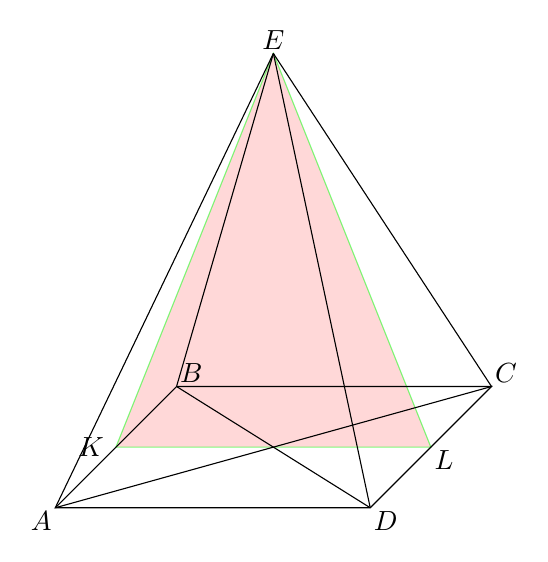
\begin{tikzpicture}[scale=1,inner sep=0.4mm]
	\coordinate (A) at (0,0,4);
	\coordinate (B) at (0,0,0);
	\coordinate (C) at (4,0,0);
	\coordinate (D) at (4,0,4);
	\coordinate (E) at (2,5,2);
	\coordinate (K) at (0,0,2);
	\coordinate (L) at (4,0,2);
	
	\filldraw [draw=green,fill=red!30!white,opacity=0.5] (E) -- (K) -- (L) -- cycle;	
	
	\draw (A) node [below left] {$A$};
	\draw (B) node [above right] {$B$};
	\draw (C) node [above right] {$C$};
	\draw (D) node [below right] {$D$};
	\draw (E) node [above] {$E$};
	\draw (K) node [left=3pt] {$K$};
	\draw (L) node [below right] {$L$};

	\draw  (A) -- (B) -- (C) -- (D) --cycle;
	\draw (B) -- (D);
	\draw (A) -- (C);
	\draw (A) -- (E);
	\draw (B) -- (E);
	\draw (C) -- (E);
	\draw (D) -- (E);	
	

\end{tikzpicture} 
\end{document}